\chapter{Introduction}

\section{Introduction}

ngscopeclient is a high performance, GPU accelerated remote user interface, signal processing, protocol analysis, and
automation tool for test and measurement equipment. It runs on all major operating systems and can interoperate with a
broad and continuously growing range of T\&M products from many vendors.

As of this writing, ngscopeclient is under active development but has not had a formal v0.1
release and should be considered alpha quality.

This is free software: you are free to change and redistribute it.
There is NO WARRANTY, to the extent permitted by law.

\section{Design Philosophy}

Users familiar with conventional benchtop oscilloscopes will notice some important distinctions between ngscopeclient
and classical DSO user interfaces. While there is an initial learning curve getting used to the different ways of doing
things, these changes allow for greater productivity and more complex analysis.

Legacy DSO user interfaces largely still imitate the front panel controls of analog CRT instruments dating back to the
mid 1940s. A single view of each waveform shows the entire acquisition on a grid with a fixed number of divisions
(emulating an etched graticule on a CRT) and both time and voltage scales are defined in terms of these divisions.
While more recent DSOs do allow math functions, protocol decodes, zooms, and so on, this archaic concept has remained.

In ngscopeclient, the acquisition record length is completely decoupled from the X axis scale of the viewport, and
there is no concept of a ``zoom" waveform or measuring time in ``divisions". Arbitrarily many views of a channel may be
created, and each may be scaled and zoomed independently. Acquisition record length and duration are controlled
separately, from the timebase properties dialog.

Similarly, vertical scale for waveforms is defined in terms of full-scale range, a far more intuitive and useful metric
than arbitrary ``divisions". While horizontal grid lines are still displayed in waveform views for convenience, their
number, spacing, and locations may change. Tall plots will have more scale divisions than short ones, and the divisions
are always located at round numbers even if this requires the grid to not be centered in the plot (Fig. \ref{y-divs})

\begin{figure}[h]
\centering
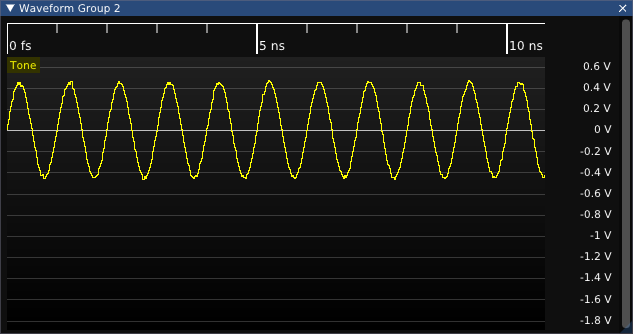
\includegraphics[width=13cm]{ng-images/y-divs.png}
\caption{Example waveform showing off-center grid and round-numbered grid lines}
\label{y-divs}
\end{figure}

Rather than optimizing for a touch screen (as is common for benchtop oscilloscopes), ngscopeclient's UI is
heavily mouse driven and context based. Space used by always-visible buttons, sliders, etc is kept to a minimum in
order to keep as much screen real estate as possible usable for waveform display. Additional controls are displayed in
menus or pop-up dialogs which can be closed, moved out of view, or docked as needed.

\section{Revision History}
\begin{itemize}
\item \today: [in progress] Initial draft
\end{itemize}
